\begin{savequote}[8cm]
Today’s young people will face a rapidly changing world of challenges on a scale unprecedented in human history. Through this ambitious program, we hope to engage tomorrow’s leaders across the globe, providing education and unique opportunities for them to identify problems, solutions, and ways they can work together, for a lifetime, in the service of humanity.”
  \qauthor{--- Wendy Schmidt}
\end{savequote}

\chapter{\label{ch:context}Decisions in the Global Talent Selection Context}
\minitoc

\section{The Social Value of Selection}\label{sec:social_value}
Scholarship programs offer long-term benefits to their chosen scholars, often under the theory that providing these benefits improves not only the welfare of the scholars themselves but of society as a whole \cite{DilraboJonbekova_Ruby_2023,Dassin_Marsh_Mawer_2018}. Theories of the mechanisms of this social benefit vary. Some theories rely on the future actions of the chosen scholars. For example, \textcite{Dassin_Marsh_Mawer_2018} argue that scholars are often empowered and disposed to devote themselves to solving global problems. \textcite{Dassin_Marsh_Mawer_2018} also note that these scholars may bring additional returns to their communities, thereby improving the welfare of a broad group of people (though they also express concern over `brain drain', where these scholars do not return to their communities). In contrast, others contend that the mere provision of scholarships to the correct recipients is itself pro-social. \textcite{minkin2023diversity} note that society benefits from making space for a breadth of perspectives; providing scholarships to those who would otherwise be unable to afford higher education may create that breadth of perspectives. Some evidence suggests that this broader range of perspectives brings additional benefits in the form of increased productivity \cite{autor2008does,noray2023systemic}. Besides the gain to organisations, though, some argue that the social mobility brought about by the existence of scholarship programs yields inherent benefit to society \cite{Dassin_Marsh_Mawer_2018}. Under any of these theories, selecting the ``best'' applicants as scholars is clearly in society's best interest. However, as we explore throughout this thesis, different theories of change yield different definitions of ``best''.

Traditional selection is a human-led process, and many suggest it should remain that way \cite{Latzer_Hollnbuchner_Just_Saurwein_2014}. However, as the number of applicants to scholarship programs grows, the need for scalable selection processes has grown; with traditional selection processes unequipped to handle these new challenges, organisations are forced to innovate, often turning to algorithmic solutions that offer to solve these difficult problems \cite{Latzer_Hollnbuchner_Just_Saurwein_2014}. This has led to the development of Decision Support Tools (DSTs) to support selection processes. These DSTs range from simple tools like automated essay scoring to more complex tools like AI-driven selection algorithms. The use of these tools is not without controversy. Critics argue that these tools may be biased \cite{dwork_fairness_2012}, or may dehumanise the selection process \cite{binns_its_2018}. However, while certain features of these tools may succumb to some critiques, evolving discussions about fairness in selection render older, human-led selection processes equally vulnerable to critique \cite{Ahnaf2023AHPAP,pmlr-v80-kearns18a}.

\section{Related Work}
This thesis engages primarily with literature seeking to use AI tools to support decision-making in global scholarship selection processes. Unfortunately (or perhaps fortunately), this particular niche of literature is fairly sparse. While many tools do exist, especially those seeking to automate the job of the scholarship selector entirely, we are forced to look beyond this niche for a larger body of related literature. Primarily, we do this by considering other selection contexts (e.g., universities or recruiters). Note that while this body of literature is large, and contains work ranging from automated essay scoring to intellect testing \cite{cozma_automated_2018,condon2014international}, our work is only tangentially related to these fields. Some work explores applicant perceptions of scholarship selection processes \textcite{10.1145/3351095.3372867}, but this work is primarily interested in the decision subjects and does not engage with the design of selection processes.

More closely related is the body of algorithmic fairness literature engaging with recruitment, much of which seeks to ensure that AI tools do not discriminate against protected classes \cite{dwork_fairness_2012}. However, as we explore in this chapter, disanalogies between recruitment and global scholarship selection limit the applicability of this work.

Similarly, much work explores the impact of algorithms on educational outcomes. For example, \textcite{NISSENBAUM1998237} explore the risk of algorithmic involvement in education dehumanising the experience. However, though these works are conducted in the same environment, they do not touch on selection itself.

This chapter also explores a model of selection as subordinate decisions and investigations supporting the ultimate decision about which subset of applicants to select as scholars. Many of these subordinate decisions relate to their own bodies of literature; these are explored in the relevant chapters.

\section{On Working with Scholarship Programs}
It is unsurprising that little research explores this unique and novel context. In part, we account this to the necessity of longitudinal research with or on organisations. And the novelty of these programs, combined with an understandable desire to avoid the scrutiny arising from public identification in research, has made research with or on these programs challenging.\footnote{Critics may point to the Rhodes Scholarship, founded in 1902, as an example of a long-standing global scholarship organisation \cite{Ziegler_2008}. However, the program's history of intentional exclusionism challenges their claim to global reach; the Rhodes Scholarship did not accept women until legally mandated in 1977 \cite{Ziegler_2008}, and continued to discriminate against Black South Africans until the legalisation of the African National Congress and the end of Apartheid in 1991 \cite{Ziegler_2008}. Furthermore, though the Rhodes Scholarship does select a range of applicants from around the world, they do so via regional committees that compare applicants from similar backgrounds, thus sidestepping the central difficulty of global selection.}

Fortunately, this thesis engages with two such organisations, \rise and \eit. Both are already seeking to embed AI and computational DSTs into their processes (e.g., \eit already uses an AI-based automated essay scoring system). Both programs have asked that they not be identified in public facing research, and thus we request that reviewers not share details on either program, and to protect the identities of the programs where possible. For more details on the programs, see Appendix \ref{app:programs}.

\begin{table}[htbp]
  \centering
  \caption{This table enumerates relevant decision points facing selectors and selection teams.}
  \label{tab:full_decision_list}
  \adjustbox{max width=\textwidth}{
  \begin{tabular}{l r p{0.33\linewidth}p{0.33\linewidth}}
      \toprule
      Decision Point & Chapter(s) & Decision Description & Supporting Information \\
      \midrule
      \emph{Salary} & \ref{ch:xai} & A program may desire to deferentially treat a person based on an estimate of their salary. & AI-calculated estimations of salary range based on census information of that individual. \\ 
      \emph{Credit} & \ref{ch:xai} & A program may desire to accept or deny a hypothetical person's loan application based on their creditworthiness. & An AI-generated prediction of whether someone will be severely delinquent in making a credit payment. \\ 
      \emph{Refinement} & \ref{ch:xai} & \rise refines its scoring algorithm each year to better score applicants. & Explanations of perplexing AI-generated scores. \\ 
      \emph{Diligence} & \ref{ch:genai} & \rise makes holistic decisions about when and how to consider applicants. & Information about which essays (and which parts of essays) were written by genAI; information about whether the genAI-written passages are hallucinations. \\ 
      \emph{Partners} & \ref{ch:genai} & \rise must determine whether to continue channel partnerships, which encourage and support applicants. & Whether any channel partners' affiliated applicants use genAI disproportionately. \\
      \emph{Pipeline} & \ref{ch:genai} & \rise decides whether to modify their application material or process. & Information about usage of genAI throughout the application pipeline. \\
      \emph{Gameability} & \ref{ch:genai} & \rise decides how to modify their application material or process. & Information about the how AI-generated essays are scored under the current application process. \\
      \emph{Disqualification} & \ref{ch:genai} & A program may decide to disqualify an applicant that violates their application guidelines. & Information about whether essays violate application guidelines around genAI usage. \\
      \emph{Diversity} & \ref{ch:diversity} and \ref{ch:spf} &\rise and \eit make cohort-level decisions regarding the diversity of their cohort. & Information about the diversity of possible cohorts. \\
      \emph{Contribution} & \ref{ch:diversity} and \ref{ch:spf} &\rise and \eit make applicant-level decisions about which applicants to move forward based on their contribution to cohort diversity. & Information about the impact of including different applicants on cohort diversity. \\
      \bottomrule
  \end{tabular}
  }
\end{table}

We engage these programs, variously, in AR, VSD, and PD. In working with the \rise and \eit programs to support solutions to the central \emph{Selection} decision point, the programs expressed interest in supporting many subordinate decision points. While some of them, such as automating the essay scoring process, fall outside the scope of this thesis, we isolate three families of decision points that engage with AI or HCI literature, and are thus of both program and research interest. These families are: decisions supported by explainable AI algorithms, decisions about applicant usage of genAI, and decisions about the diversity of selected cohorts. Table \ref{tab:full_decision_list} enumerates decision points of interest to us. 

\section{The Decision Matrix: A Framework for Understanding Selection Decisions and Evaluating DSTs}
In Chapter \ref{ch:genai}, we uncover through a process of AR a framework we term the \emph{Decision Matrix}. Though this framework is completed in this chapter, a shadow of this framework can be found in Chapter \ref{ch:xai}, and the axes of the framework are central to understanding the relevance of each chapter to the thesis as a whole. Thus, we present the framework here.

The \emph{Decision Matrix} framework sees us identifying ``decision points'' that selectors and selection teams are faced with categorising them on two axes: \emph{stage} and \emph{stakes}. The \emph{stage} axis captures the important distinctions between decisions made in the process of selection (\emph{in-process}) and decisions made \emph{ex-post}, after the primary \emph{Selection} decision of ``What cohort of people do we select?'' has been made. The \emph{stakes} axis, in contrast, captures the sensitivity (or severity) of the decisions. E.g., choosing to disqualify or select and applicant is a \emph{high-stakes} decision, while choosing to assign extra staff to evaluate the truthfulness of an applicant's claims is a comparatively \emph{low-stakes} decision.

Chapters \ref{ch:xai}, \ref{ch:diversity}, and \ref{ch:spf} do not make explicit mention of the Decision Matrix framework, but are nonetheless influenced by the placement of the relevant decision points on the matrix. We make the distinction between \emph{in-process} and \emph{ex-post} in Chapters \ref{ch:xai} and \ref{ch:genai}, where we evaluate two different pre-existing decision support paradigms for scholarship selection. In both chapters, we find the paradigms suited to \emph{ex-post} decision support, but lacking for \emph{in-process} decisions.\footnote{Note that Chapter \ref{ch:xai} does not explicitly discuss the \emph{Salary} and \emph{Credit} decision point as they are listed here. The framing in Chapter \ref{ch:xai} was presented to study participants, while the framing here is most interesting from our perspective.} Thus, Chapters \ref{ch:diversity} and \ref{ch:spf} aim to construct a DST suitable for supporting \emph{in-process} decisions. As many of the social motivations for scholarship programs listed in Chapter \ref{sec:social_value} rely on selecting diverse groups of scholars, these chapters seek to support decision points related to the diversity of the cohort of selectors. Figure \ref{fig:full_decision_matrix} places relevant decision points from Table \ref{tab:full_decision_list} on the Decision Matrix.

\begin{figure}[htbp]
  \centering
  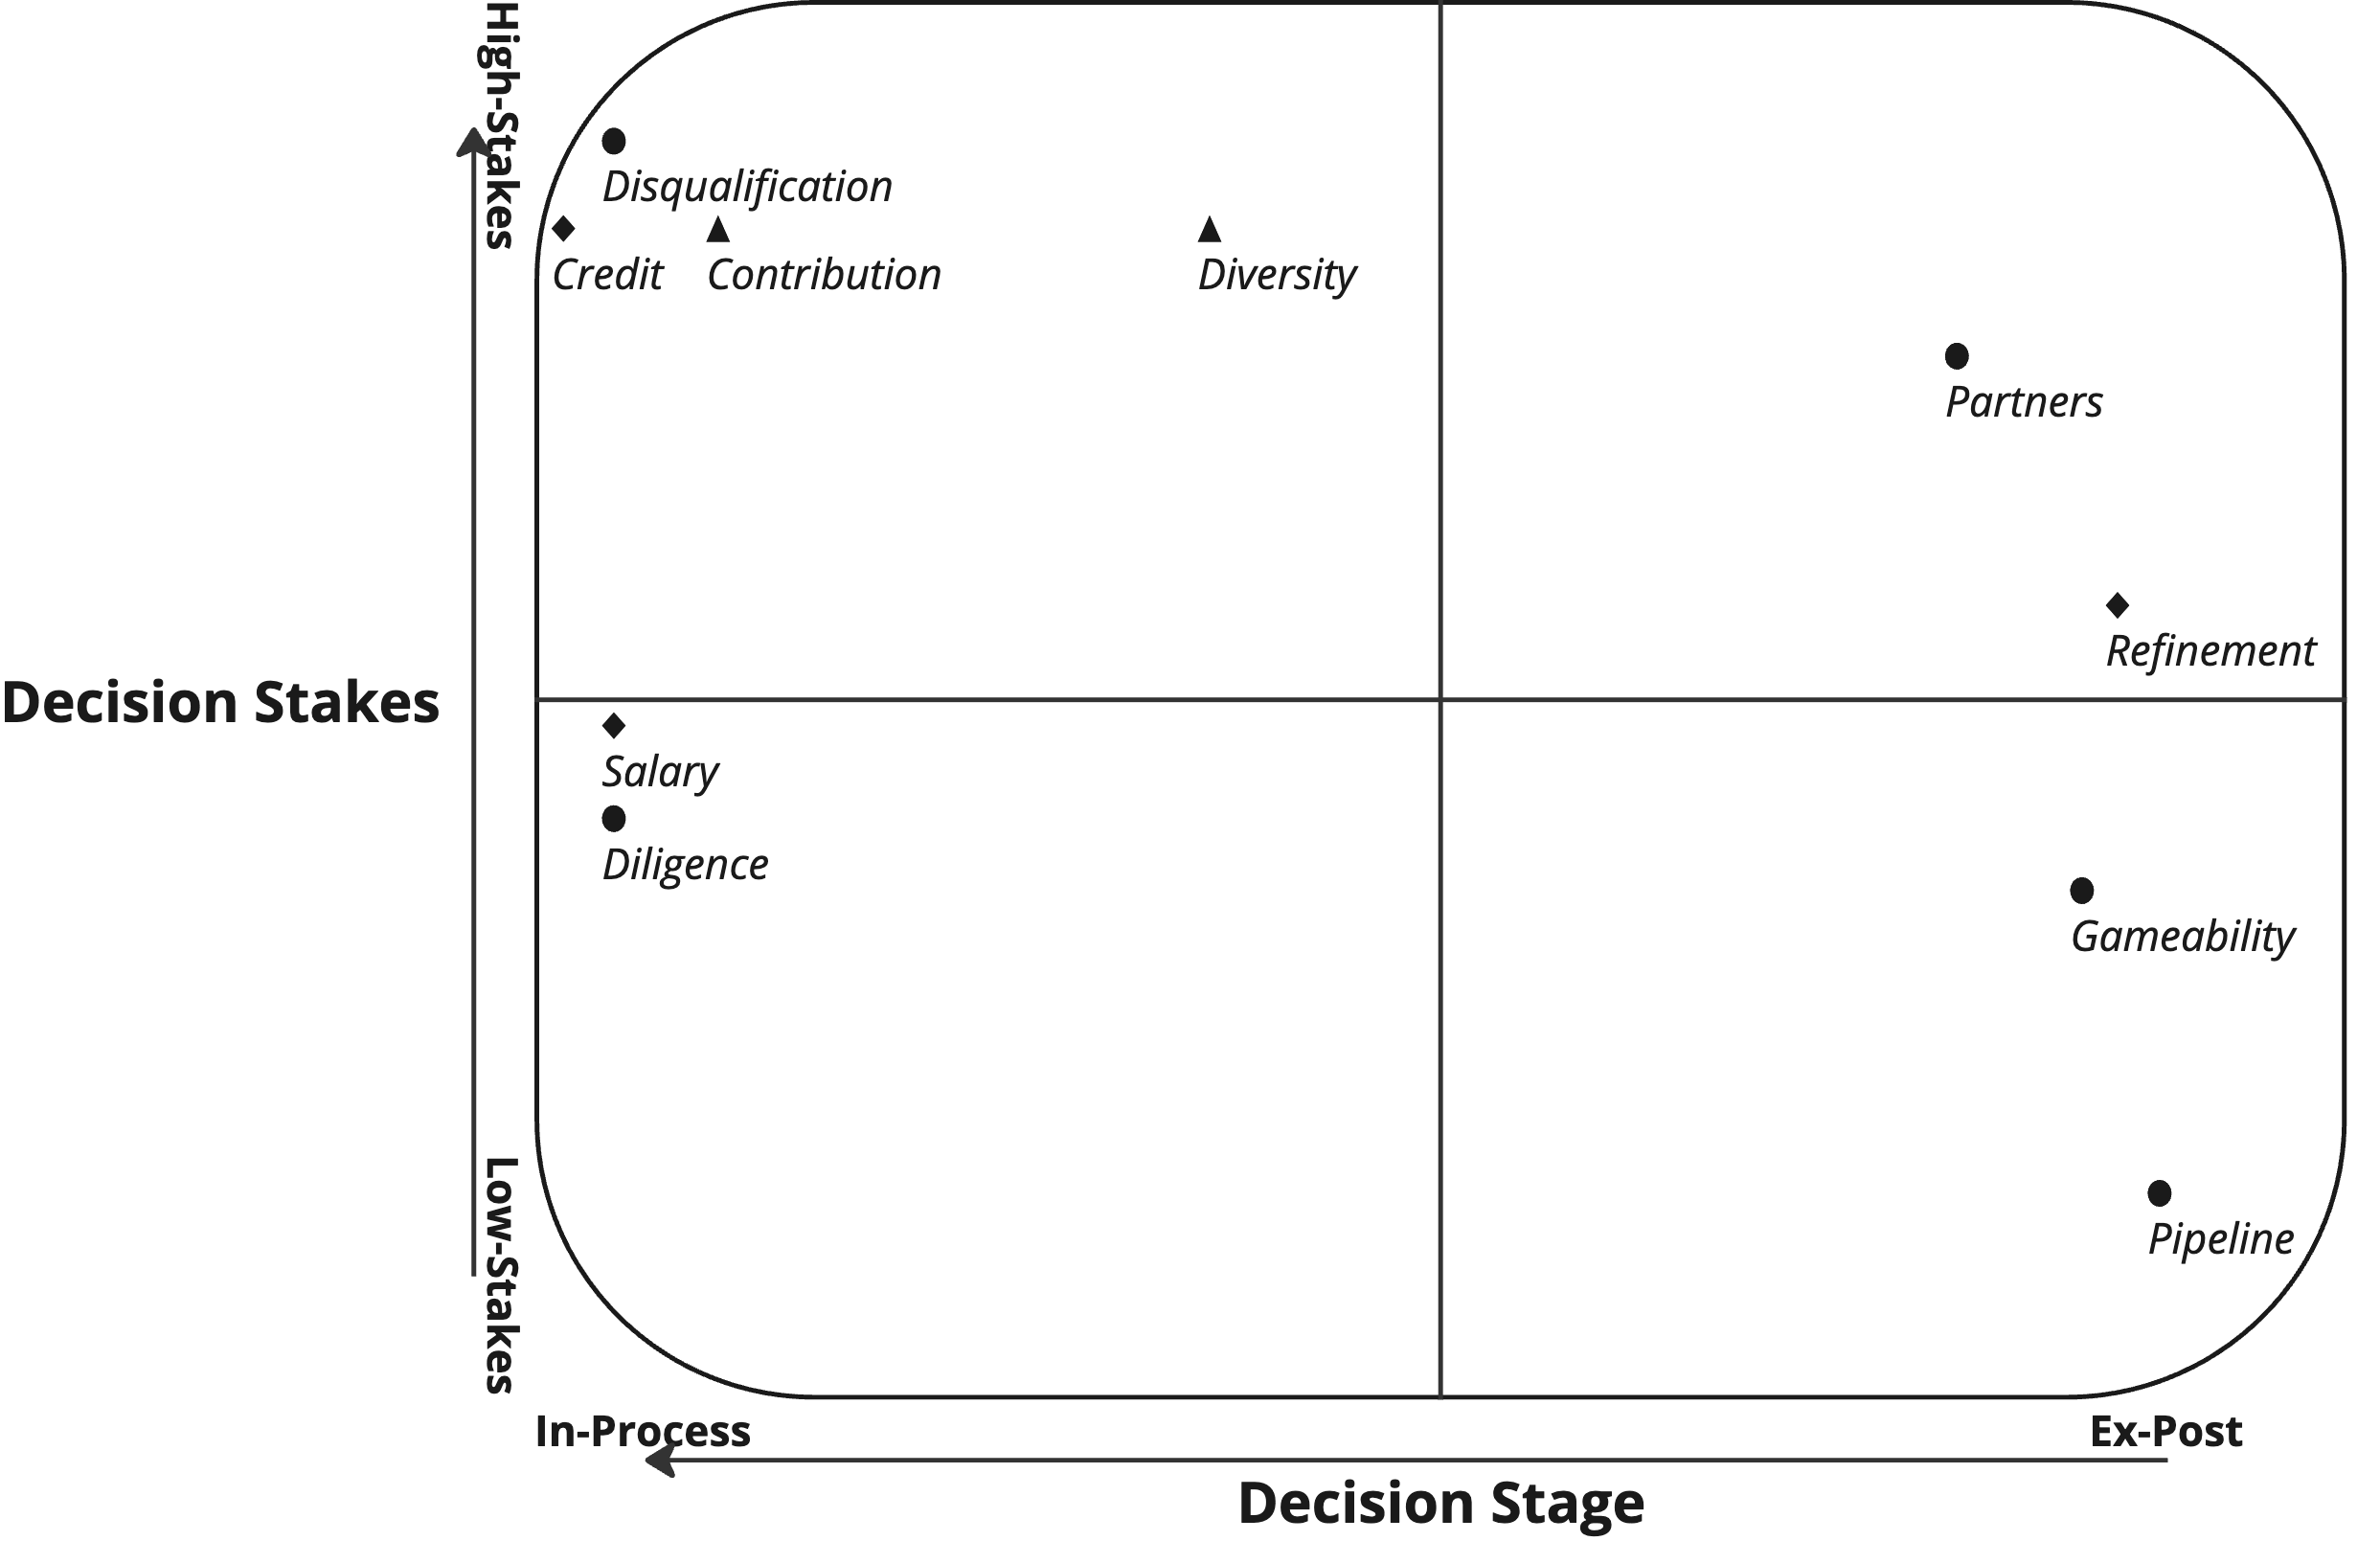
\includegraphics[width=0.8\textwidth]{context/full_decision_matrix.png}
  \caption{This figure places the decisions from Table \ref{tab:full_decision_list} on the Decision Matrix.}
  \label{fig:full_decision_matrix}
\end{figure}